


Geomecânica é o estudo das deformações e tensões em solos e rocha. Esse estudo se torna de extrema importância, pois, várias problemas podem ser solucionados através desses estudos, como:
\begin{itemize}
    \item Cálculo da pressão de fratura.
    \item Estabilidade de poços
\end{itemize}

Assim, simulações de geomecânicas são importantes para uma exploração segura do campo.

\section{Tensor de Tensões}

Para representar a tensão em um ponto da rocha, é utilizado um tensor de tensões de segunda ordem como segue abaixo:

\begin{equation}
\mathbf{\sigma} =
    \begin{bmatrix}
    \stxx & \stxy & \stxz \\
    \styx & \styy & \styz \\
    \stzx & \stzy & \stzz 
    \end{bmatrix}
\end{equation}

O primeiro subscrito do tensor representa a face que a tensão está sendo aplicada, enquanto o segundo representa a direção da tensão. A figura \ref{fig:tensoesx} mostra as componentes com o com primeiro subscrito x.


\begin{figure}[!htbp]
\label{fig:tensoesx}
\centering
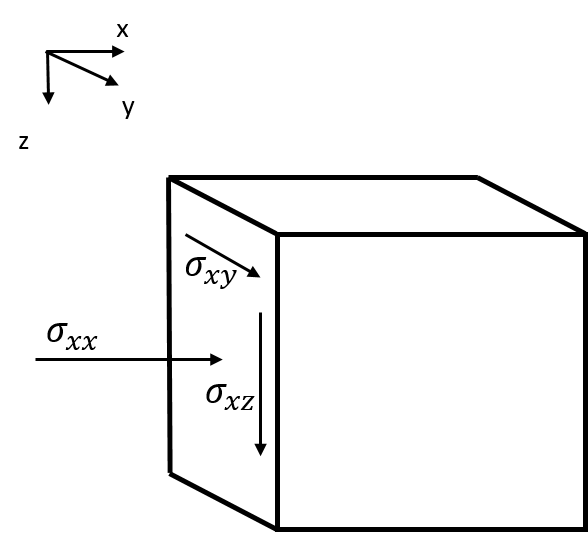
\includegraphics[width=5cm]{chap01/tensor.png}
\caption{Tensões $\sigma_{x.}$ representadas graficamente.}
\end{figure}

Ao aplicar a condição de equilíbrio do momento, chega-se a conclusão que $\stxy=\styx$, $\stxz=\stzx$ e $\styz=\stzy$. Dessa maneira, para a representação desse tensor, são necessários guardar apenas seis valores.
\begin{equation}
\label{eq:tensor6}
\sigma^T = \begin{bmatrix}
\stxx & \styy & \stzz & \stxy & \stxz & \styz
\end{bmatrix}
\end{equation}

Para o cálculo da tensão exercida é um determinado plano, basta multiplicar o tensor de tensão por um vetor ortonormal ao plano desejado de maneira que:

\begin{equation}
T = 
\end{equation}


\section{Teoria da Consolidação}

Para um certo elemento de volume $\Delta x\Delta y \Delta z$, representado na figura \ref{fig:equilibrio}, pode-se escrever o equilíbrio nas direções x, y e z.

\begin{figure}[!htbp]
\label{fig:equilibrio}
\centering
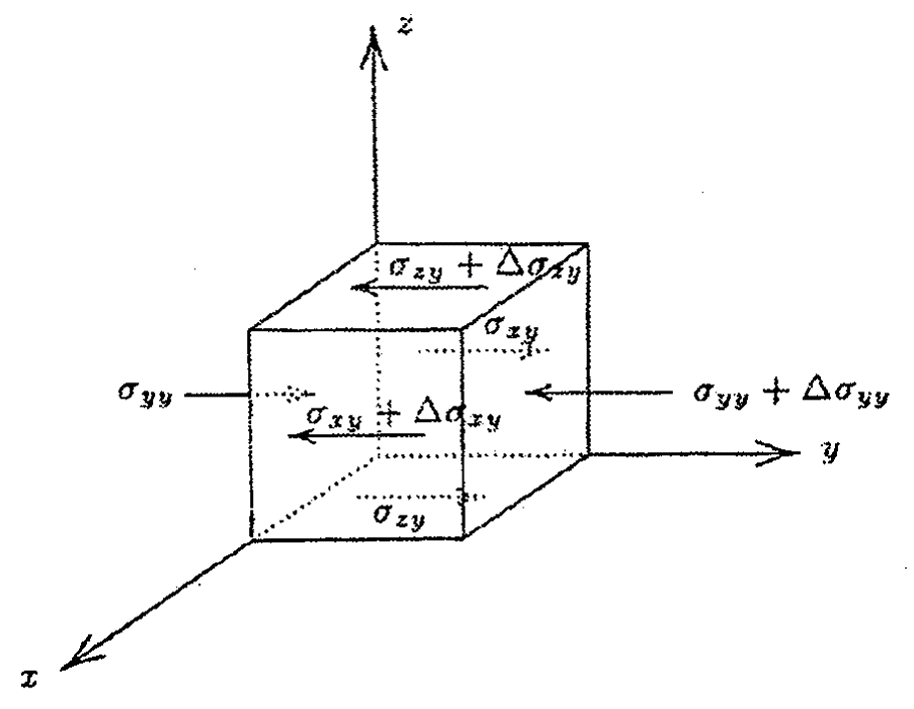
\includegraphics[width=6cm]{chap01/equilibrio.png}
\caption{Tensões na direção y ($\sigma_{.y}$) representadas graficamente.  Fonte: \cite{CompGeomec}}
\end{figure}

Para a direção y, por exemplo, tem-se:

\begin{multline}
   (\stxy - \stxy - \Delta \stxy) \Dy\Dz + (\styy - \styy - \Delta \styy)\Dx\Dz  +\\
   + (\stzy - \stzy - \Delta\stzy) \Dx\Dy + f_y\Dx\Dy\Dz = 0 
\end{multline}

\begin{equation}
 \Delta \stxy \Dy\Dz + \Delta \styy\Dx\Dz + \Delta\stzy - f_y\Dx\Dy\Dz = 0
\end{equation}

\begin{equation}
\dx[\stxy] + \dy[\styy] + \dy[\stzy] - f_y = 0
\end{equation}

Analogamente, para as outras direções, pode-se montar o seguinte sistema de equações de equilíbrio.

\begin{equation}
\label{eq:equilibrio1}
\left\{\begin{matrix}
 \dx[\stxx] + \dy[\styx] + \dz[\stzx] - f_x & = & 0\\ 
 \dx[\stxy] + \dy[\styy] + \dz[\stzy] - f_y & = & 0\\ 
 \dx[\stxz] + \dy[\styz] + \dz[\stzz] - f_z & = & 0
\end{matrix}\right.
\end{equation}

As tensões apresentadas nas equações \ref{eq:equilibrio1} são as atuam no bloco infinitesimal. Acontece que ao tratar de reservatórios de petróleo, estes possuem fluído no volume poroso da rocha (óleo ou água) e, portanto, parte da tensão será suporta pelo fluído e parte será suportado pelos grãos da rocha. Como fluído não oferece resistência ao cisalhamento, ele suporta apenas parte das tensões $\stxx$, $\styy$ e $\stzz$.

Experimentalmente foi constado que a equação que rege a tensão efetiva na rocha ($\sigma^\prime$) é dada pela equação \ref{eq:tensaoefetiva} (veja \cite{ResGeomec} cap 02). 

\begin{equation}
\label{eq:tensaoefetiva}
    \sigma^\prime = \sigma - \alpha P_p
\end{equation}

Onde $\alpha$ é o coeficiente de biot e $P_p$ a pressão de poros. O coeficiente de biot representa o quanto a pressão de poros do fluído suporta a tensão total na rocha, portanto, $\alpha \in [0,1]$.

Assim, as equações \ref{eq:equilibrio1} podem ser reescritas como \ref{eq:equilibrio} substituindo a tensão total $\sigma$ pela tensão efetiva na rocha ($\sigma^\prime$). Essas equações são encontras em \cite{CompGeomec}.



\begin{equation}
\label{eq:equilibrio}
\left\{\begin{matrix}
\dx[\sxx]  + \dy[\syx] + \dz[\szx] + \dx[\alpha P_p] - f_x   = 0
\\
\dx[\sxy]  + \dy[\syy] + \dz[\szy] + \dy[\alpha P_p]  - f_y   = 0
\\
\dx[\sxz]  + \dy[\syz] + \dz[\szz] + \dz[\alpha P_p] - f_z   = 0
\end{matrix}\right.
\end{equation}

Ou ainda, escrevendo de forma matricial. 

\begin{equation}
\label{eq:equilibrio_matriz}
\nabla \cdot \sigma^\prime + \nabla \alpha P_p - f = 0
\end{equation}

Onde $f^T=\begin{bmatrix}f_x & f_y & f_z\end{bmatrix}$.


Por motivos de implementação mais eficiente (uso de menos memória), é interessante reescrever as equações utilizando a notação do tensor de tensões apenas com seis elementos como na equação \ref{eq:tensor6}. Portanto, considerando os seguintes operadores e vetores.

\begin{equation}
\begin{matrix}
\sigma^\prime = \begin{bmatrix}
\sxx
\\
\syy
\\
\szz
\\
\sxy
\\
\sxz
\\
\syz
\end{bmatrix}
&

;

&

f = \begin{bmatrix}
f_{x}
\\
f_{y}
\\
f_{z}
\end{bmatrix}
&
;
&

P = \begin{bmatrix} P_p \\ P_p \\ P_p \\0 \\ 0 \\ 0\end{bmatrix}

&
;

&
S = \sop
\end{matrix}
\end{equation}

A equação \ref{eq:equilibrio_matriz} pode ser reescrita como \ref{eq:equilibrio_final}. Essa equação será discretizada na próxima sessão através do método dos elementos finitos.

\begin{equation}
\label{eq:equilibrio_final}
S^T\sigma^\prime + S^T\alpha P - f = 0
\end{equation}


\subsection{Relações Constitutivas}

\textit{"Uma relação constitutiva descreve a deformação de uma rocha em resposta a uma tensão (e vice-versa)."} \cite{ResGeomec}


Vários tipos de leis constitutivas podem ser utilizadas para representar essa relação entre tensão e deformação. A figura \ref{fig:stress_strain} mostram dados de um teste típico de tensão-deformação em uma rocha bem cimentada. Nesse caso, é importante notar que o comportamento linear é a região dominante nesse tipo de teste. Essa região onde as deformações e tensões se relacionam linearmente é chamada de elástica.


\begin{figure}[!htbp]
\label{fig:stress_strain}
\centering
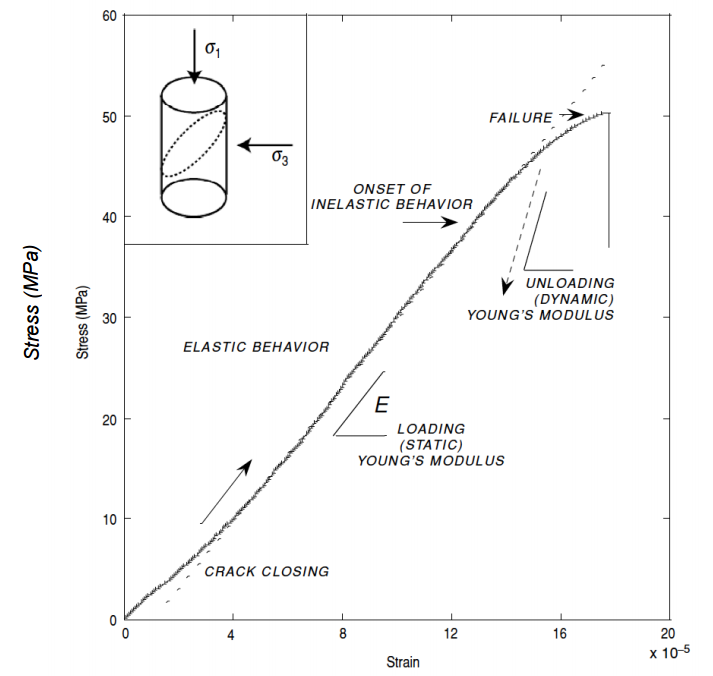
\includegraphics[width=7cm]{chap01/stress_strain.PNG}
\caption{Teste de laboratório tensão-deformação para uma rocha bem cimentada. Fonte: \cite{ResGeomec}}
\end{figure}


O estudo de mecânica dos sólidos nos mostra que, na região elástica e materiais isotrópicos, é possível escrever uma relação entre as deformações e tensões nos elementos de forma simples. Essa relação é denominada de Lei de Hooke Generalizada e é apresentada na equação \ref{eq:hooke}.


\begin{equation}{
\label{eq:hooke}
\fontsize{4}{4}\selectfont
\stvetor = \elastic \evetor
}
\end{equation}

Onde $E$ é o módulo de Young da rocha e $v$ o módulo de de Poisson. 

Já as deformações se relacionam com os deslocamentos pela equação \ref{eq:defor_desloc}.

\begin{equation}
\label{eq:defor_desloc}
\evetor = \sop \uvetor
\end{equation}

\begin{equation}
\label{eq:defor_desloc2}
\evetor = S \uvetor
\end{equation}

A EDP da equação \ref{eq:equilibrio_final} pode então ser escrita em função dos deslocamentos substituindo as equações \ref{eq:hooke} e \ref{eq:defor_desloc2}.

\begin{equation}
\label{eq:edp_geomec}
S^TDS u + S^T\alpha P - f = 0
\end{equation}

Onde $D$ é a matriz de elasticidade da Lei de Hooke. Essa forma será a utilizada junto dos métodos do elementos finitos para construção do simulador.



\section{Modelagem pelo Método dos elementos finitos}

Em posse da equação \ref{eq:edp_geomec}, é necessário um método de solução de EDP's. O método utilizado no simulador em questão é dos elementos finitos. O método do elementos finitos é bastante utilizado em problemas de elasticidade. {\color{red}TODO: Achar referencia sobre tópicos de elementos finitos.}


\subsection{Divisão do domínio}

O domínio do problema será dividido em uma quantidade finita de elementos. Os elementos considerados na formulação serão elementos hexaédricos. Outros tipos de elementos podem ser considerados mas o simulador em questão utiliza apenas elementos desse formato. Dessa maneira, os elementos tem a forma mostrada na figura \ref{fig:elemento}.


\begin{figure}[!htbp]
\label{fig:elemento}
\centering
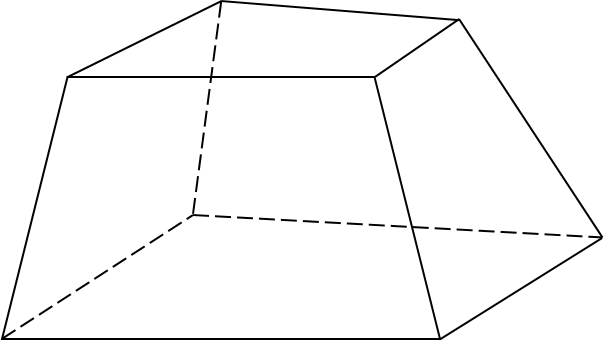
\includegraphics[width=5cm]{chap01/elemento_original.png}
\caption{Elementos de divisão do domínio.}
\end{figure}

Para esse tipo de elemento a quantidade de vértices é oito. Para o problema, cada vértice terá 3 graus de liberdade, pois cada um deles pode se mover em três direções (x, y, z). Assim, o campo vetorial $u$ será aproximado pelos valores no nós e fora deles por uma interpolação dos valores dos nós como a equação \ref{eq:udiscret}.


\begin{equation}\label{eq:udiscret}
u(\mathbf{x}) = \sum_{i=1}^{nn} \varphi_i(\mathbf{x}) * \begin{bmatrix}
u^i_x \\ u^i_y \\ u^i_z
\end{bmatrix}
\end{equation}

Onde $u^i_x$, $u^i_y$ e $u^i_z$ são os graus de liberdade do nó i. As funções $\varphi_i(\mathbf{x})$ são tais que o valor no nó correspondente é igual a 1 e descresce para 0 nos nós adjacentes. A forma dessas funções serão definidas mais a frente, pois elas são definidas em um sistema diferente do (x,y,z).


Considerando $u^*$ como a solução exata para a EDP \ref{eq:edp_geomec} é necessário encontrar a função $u$ da forma de \ref{eq:udiscret} que aproxime da melhor maneira possível $u^*$ de acordo com alguma métrica. Uma maneira de fazer isso é minimizar a norma do resíduo $r = u-u^*$. Para essa minimização, o resíduo  deve ser ortogonal a cada uma das funções $\varphi_i$ e as equações apresentadas em \ref{eq:normalizacao} são válidas.


\begin{equation}\label{eq:normalizacao}
<u-u^*, \varphi_i> = 0   \quad  \text{para $i$=1,2,3, ..., nn}
\end{equation}

A definição da norma que será utilizada aqui é de extrema importância, note que, caso a norma canônica for utilizada, nada pode ser feito com relação a equação \ref{eq:normalizacao} pois, nos problemas práticos, geralmente não se conhece $u^*$.

\begin{equation}
    <f(x), g(x)> = \int^b_af(x)g(x) dx
\end{equation}

Como apresentado em \cite{CompGeomec} mais detalhadamente, o método de garlekin minimiza o módulo do resíduo na norma da energia. De forma que, o produto interno utilizado é o apresentado na equação \ref{eq:proint_energia}.



\begin{equation}
\label{eq:proint_energia}
<u-u^*, \varphi_i> = \omeint{(S^T\,D\,S(\mathbf{u - u^*})) \phiix} \quad \text{para $i$=1,2,3, ..., nn}
\end{equation}

Assim, é possível rearrumar cada uma das equações da seguinte maneira:


\begin{equation}
\omeint{(S^T\,D\,S(\mathbf{u - u^*})) \phiix}  =  \omeint{(S^TDSu)\phiix} - \omeint{(S^TDSu^*)\phiix}              
\end{equation}

É possível remover $u^*$ da equação utilizando \label{eq:edp_geomec} chegando em uma equação dependendo apenas dos graus de liberdade $u^i_x$, $u^i_y$ e $u^i_z$.

\begin{equation}
\omeint{(S^T\,D\,S(\mathbf{u - u^*})) \phiix}  =  \omeint{(S^TDSu)\phiix} + \omeint{\mathbf{F}\phiix} \quad \forall     
\end{equation}

\begin{equation}
\omeint{(S^TDSu)\phiix} + \omeint{\mathbf{F}\phiix} = 0
\end{equation}

\begin{equation} \label{eq:garlekin}
\omeint{(S^TDSu)\phiix} = - \omeint{\mathbf{F}\phiix}
\end{equation}



Os próximos passos serão para transformar \ref{eq:garlekin} em uma forma mais simples para resolução. 

\begin{equation}
\omeint{S^T\,D\,S\mathbf{u} \phiix} = \omeint{S^T\sigma \phiix}
\end{equation}

\begin{equation}
\omeint{S^T\sigma \phiix} = \omeint{\sstensor \phiix} 
\end{equation}

Definindo, $\sigma_x = (\sigma_{xx}, \sigma_{xy}, \sigma_{xz})$, $\sigma_y = (\sigma_{yx}, \sigma_{yy}, \sigma_{yz})$ e $\sigma_z = (\sigma_{zx}, \sigma_{zy}, \sigma_{zz})$.

\begin{equation}\label{eq:grad}
\omeint{\sstensor \phiix} = \omeint{
\begin{bmatrix}
\nabla \sigma_x \phiix\\ \nabla \sigma_y \phiix \\ \nabla \sigma_z \phiix
\end{bmatrix}}
\end{equation}

Mas a propriedade do divergente apresentada em \ref{eq:intpartes} é válida para $f:\mathbb{R}^n \rightarrow \mathbb{R}^n$ e $g:\mathbb{R}^n \rightarrow \mathbb{R}$.

\begin{equation} \label{eq:intpartes}
\nabla (f(x)g(x)) = (\nabla f(x)) g(x) + f(x)\nabla g(x)
\end{equation}


Portanto, pode-se utilizar a seguinte equação em \ref{eq:grad}.

\begin{equation}
\nabla \sigma_x \phiix = \nabla (\sigma_x \phiix) - \sigma_x \nabla \phiix
\end{equation}


\begin{equation}
\omeint{
\begin{bmatrix}
\nabla \sigma_x \phiix\\ \nabla \sigma_y \phiix \\ \nabla \sigma_z \phiix
\end{bmatrix}} = \omeint{
\begin{bmatrix}
\nabla (\sigma_x \phiix)\\ \nabla (\sigma_y \phiix) \\ \nabla (\sigma_z \phiix)
\end{bmatrix}
-
\begin{bmatrix}
 \sigma_x \nabla \phiix\\  \sigma_y \nabla \phiix \\  \sigma_z \nabla \phiix
\end{bmatrix}
}
\end{equation}

Na primeira parcela da integral pode ser utilizado o teorema do divergente. 



\begin{equation}
\omeint{
\begin{bmatrix}
\nabla (\sigma_x \phiix)\\ \nabla (\sigma_y \phiix) \\ \nabla (\sigma_z \phiix)
\end{bmatrix}
}
=
\iint\limits_{\partial \Omega} \sigma \phiix \: . \: \mathbf{\hat{n}} \: dS
\end{equation}

Para condições de contorno de Neumman e Dirichlet, esse termo se anula, pois:

\begin{equation*}
    u = 0 \rightarrow \sigma = 0 \rightarrow \iint\limits_{\partial \Omega} \sigma \phiix \: . \: \mathbf{\hat{n}} \: dS
\end{equation*}

\begin{equation*}
     \sigma = 0 \rightarrow \iint\limits_{\partial \Omega} \sigma \phiix \: . \: \mathbf{\hat{n}} \: dS
\end{equation*}

Caso as condições de contorno do problema não sejam homogêneas, esse termo deve ser contabilizado no lado direito do sistema do linear.

A equação do problema fica, portanto:

\begin{equation}
\omeint{
\begin{bmatrix}
 \sigma_x \nabla \phiix\\  \sigma_y \nabla \phiix \\  \sigma_z \nabla \phiix 
\end{bmatrix}}
= \omeint{\mathbf{F}\phiix}
\end{equation}


Substituindo os gradientes da equação pelo operador S e o valor das tensões $\sigma$ pela relação constitutiva.

\begin{equation}
\omeint{S^T \phiix D\,S\mathbf{u} } 
= \omeint{\mathbf{F}\phiix}
\end{equation}

Ainda é possível substituir $\mathbf{u}$ pela discretização da equação \ref{eq:udiscret}.

\begin{equation}\small
\omeint{S^T \phiix D\,S \sum_{j=1}^{nn}  \phijx
 * \begin{bmatrix} u^j_x \\ u^j_y \\ u^j_z \end{bmatrix}
}   =  \omeint{\mathbf{F}\phiix} \quad \forall \: i=1,...,nn
\end{equation}


\begin{equation}\small
\sum_{j=1}^{nn} \omeint{S^T \phiix D\,S   \phijx
 * \begin{bmatrix} u^j_x \\ u^j_y \\ u^j_z \end{bmatrix}
}   =  \omeint{\mathbf{F}\phiix} \quad \forall \: i=1,...,nn
\end{equation}

O próximo passo, é dividir a integral para cada um dos elementos que o domínio foi dividido. 

\begin{equation*}\small
\sum_{j=1}^{nn} \sum\limits_e \omeeint{S^T \phiix D\,S  \phijx
 * \begin{bmatrix} u^j_x \\ u^j_y \\ u^j_z \end{bmatrix}
}   =  \sum\limits_e \omeeint{\mathbf{F}\phiix}
\end{equation*}
\begin{equation*}
 \quad \forall \: i=1,...,nn
\end{equation*}

Definindo,

\begin{equation} \label{eq:ae_def}
 a_e(\phiix,\phijx) := \omeeint{S^T\phiix D S\phijx}  
\end{equation}

e

\begin{equation}
\ldint := \omeeint{\mathbf{F}\phiix}
\end{equation}

Tem-se,

\begin{equation}\small
\sum\limits_e \sum_{j=1}^{nn} a_e(\phiix,\phijx)  * \begin{bmatrix} u^j_x \\ u^j_y \\ u^j_z \end{bmatrix}  
=  \sum\limits_e \ldint \quad \forall \: i=1,...,nn
\end{equation}


Pode-se transformar o somatório em $j$ pela multiplicação de uma matriz $3\times3nn$ por uma $3nn\times1$.

\begin{equation}\small
\sum\limits_e  \begin{bmatrix} \aelinha \end{bmatrix}  * \libvetor
=  \sum\limits_e \ldint \quad 
\end{equation}
\begin{equation*}
  \forall \: i=1,...,nn   
\end{equation*}


Como a equação é válida para todo $i=1,...,nn$, é possível juntar todas as equações da forma apresentada em \ref{eq:sistemalinear}.

\begin{equation}\scriptstyle
\sum\limits_e\aemat\libvetor = \sum\limits_e \begin{bmatrix}
\ldint[1] \\
\ldint[2] \\
\vdots    \\
\ldint[nn]
\end{bmatrix}
\label{eq:sistemalinear}
\end{equation}

É importante notar que essa equação apresenta um sistema linear onde as variáveis desconhecidas são os deslocamentos de cada nó. Sobre esse sistema, as seguintes propriedades são necessárias.

\begin{itemize}
    \item A matriz é simétrica. Pois, 
    
    \begin{eqnarray}
    a_e(\phiix,\phijx)^T & = & (\omeeint{S^T\phiix D S\phijx})^T \\
                         & = & \omeeint{(S\phijx)^T D^T (S^T\phiix)^T} \\
                         & = & \omeeint{(S^T\phijx) D S \phiix} \\
                         & = & a_e(\phijx,\phiix) 
    \end{eqnarray}    
    
    \item A matriz é esparça. Cada uma das funções de forma é não nula apenas nos elementos em que aquele nó é vértice. No caso de uma malha de hexaedros, cada função de forma é não nula em oito elementos apenas. 
    
    \item A matriz é positiva definida. {\color{red}TODO: adicionar argumento que a matriz é positiva definida.}
\end{itemize}

Com a forma do sistema linear montado, resta calcular as entradas da matriz e o vetor do lado direito.

Para o cálculo da matriz, o somatório presente em \ref{eq:sistemalinear} sugere um loop em cada um dos elementos. A figura \ref{fig:elem_func_form_local} mostra um elemento com as funções de forma com numeração local. Nesse caso, apenas oito funções de forma tem valores diferentes de zero nesse domínio. 

\begin{figure}[!htbp]
\label{fig:elem_func_form_local}
\centering
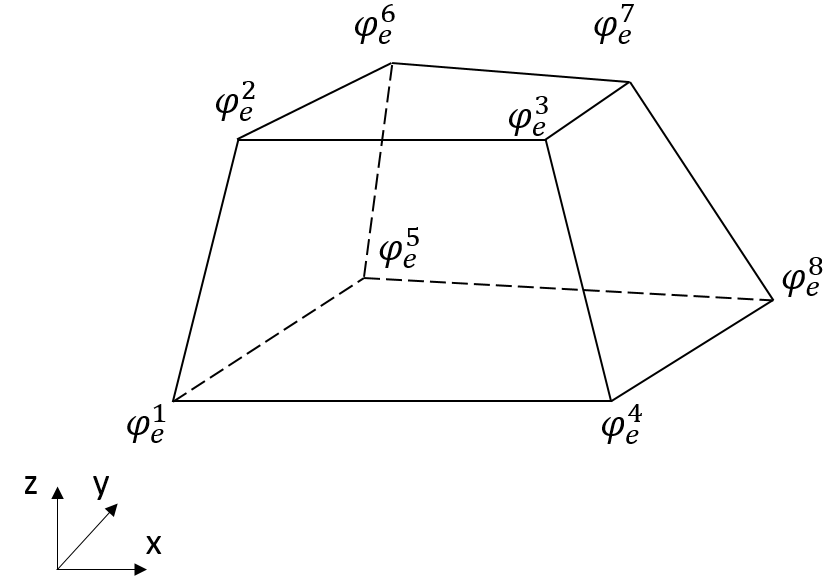
\includegraphics[width=6cm]{chap01/elemento_original_func_forma.png}
\caption{Funções de forma (numeração local).}
\end{figure}


Considere a numeração local da figura \ref{fig:elem_func_form_local}. Nesse caso, o sobrescrito $e$ nos indica que a numeração que está sendo utilizada é a local do elemento. Considerando, por exemplo, a malha $2\times2\times2$ apresentada em \ref{fig:grid2x2_elem3_vermelho}. O elemento 4 aparece em destaque com os nós pertencentes a ele em vermelho. Nesse caso, comparando com a figura \ref{fig:elem_func_form_local} pode-se associar as numerações da seguinte maneira:

\begin{itemize}
   \item $\varphi^4_1=\varphi_{17}$ em $\Omega^e$   
   \item $\varphi^4_2=\varphi_{8}$ em $\Omega^e$  
   \item $\vdots$
   \item $\varphi^4_7=\varphi_{14}$ em $\Omega^e$  
   \item $\varphi^4_8=\varphi_{11}$ em $\Omega^e$ 
\end{itemize}



\begin{figure}[!htbp]
\label{fig:grid2x2_elem3_vermelho}
\centering
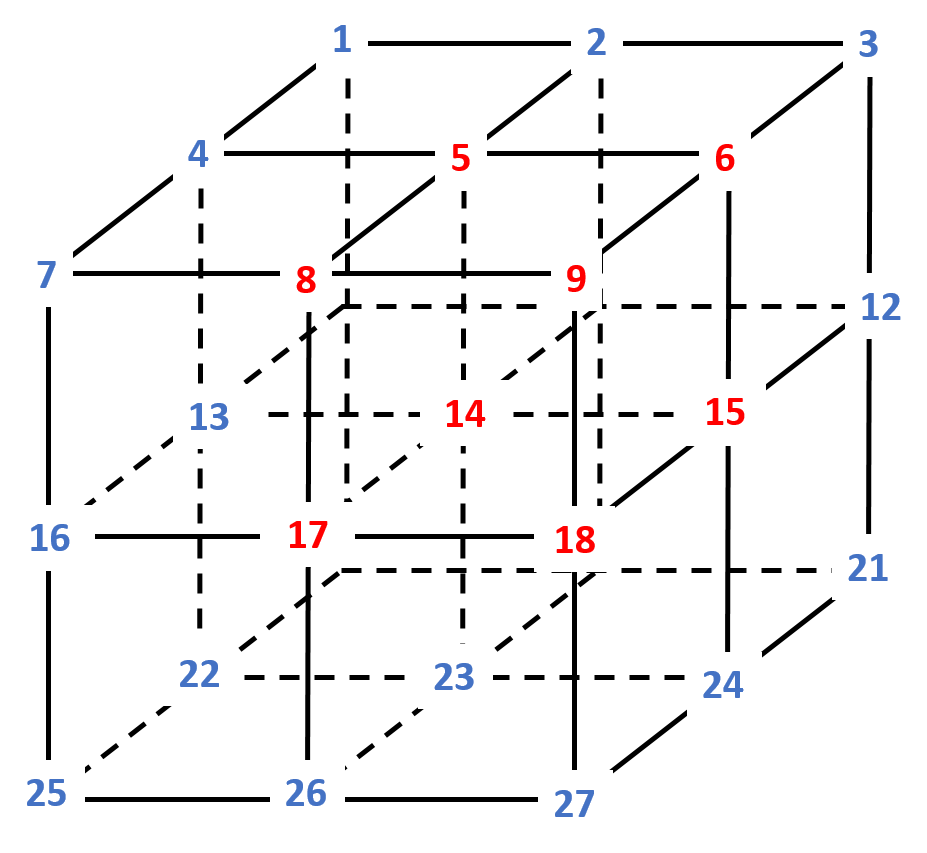
\includegraphics[width=6cm]{chap01/grid2x2_elem3_vermelho.png}
\caption{Numeração dos nós em malha $2\times2\times2$. Com elemento 4 destacado em vermelho.}
\end{figure}


Além disso, definindo $\mathbf{x^e_i} = (x^e_i, y^e_i, z^e_i)$ como as coordenadas do nó $i$ do elemento $e$ e $\Omega^e$ o domínio do elemento $e$.



Define-se como matriz do elemento, a matriz que contem apenas os valores não nulos de $a_e(\phijx,\phiix)$ no elemento. A matriz de um elemento genérico $e$ é mostrada em \ref{eq:matrizelem}.

\begin{equation}
\label{eq:matrizelem}
A^e = \aematelem
\end{equation}


Ainda falta uma definição para o valor as funções de forma. De maneira a interpolar o valor da solução $u^*$ nos nós, as funções $\phiix$ irão satisfazer as seguintes propriedades.

\begin{itemize}
\item \begin{equation}\label{eq:func_cond1}
\varphi^e_i(\mathbf{x}^e_j) = \left\{\begin{matrix} 1, \text{ se i = j} \\  0, \text{ caso contrário} \end{matrix}\right.
\end{equation}
\item \begin{equation}\label{eq:func_cond2}
    \sum_{i=1}^8 \phiix = 1
\end{equation}
\end{itemize}


O fato é que definir tais funções nos domínios $\Omega^e$ é uma tarefa complicada. Além disso, a expressão de $a^e(\phiix,\phijx)$ envolve integrais que são mais complicadas em um domínio {\color{red}``irregular''} como $\Omega^e$.


Assim, para o facilitar a definição das funções de forma e do cálculo das integrais pode-se fazer uma mudança para um elemento base $\xi$ definido em $\Omega^\xi = [-1,1]\times[-1,1]\times[-1,1]$. As variáveis que irão indicar as coordenadas nesse novo domínio são $\xi$, $\eta$ e $\zeta$. As funções de base $N_i$ no elemento base são definidas em $\Omega^\xi$ são apresentadas em \ref{eq:func_base}.

\begin{equation}
\begin{matrix}\label{eq:func_base}
N_1(\xi, \eta, \zeta) = \frac{1}{8} (1-\xi)(1-\eta)(1-\zeta) \\
N_2(\xi, \eta, \zeta) = \frac{1}{8} (1-\xi)(1-\eta)(1+\zeta) \\
N_3(\xi, \eta, \zeta) = \frac{1}{8} (1+\xi)(1-\eta)(1+\zeta) \\
N_4(\xi, \eta, \zeta) = \frac{1}{8} (1+\xi)(1-\eta)(1-\zeta) \\
N_5(\xi, \eta, \zeta) = \frac{1}{8} (1-\xi)(1+\eta)(1-\zeta) \\
N_6(\xi, \eta, \zeta) = \frac{1}{8} (1-\xi)(1+\eta)(1+\zeta) \\
N_7(\xi, \eta, \zeta) = \frac{1}{8} (1+\xi)(1+\eta)(1+\zeta) \\
N_8(\xi, \eta, \zeta) = \frac{1}{8} (1+\xi)(1+\eta)(1-\zeta)
\end{matrix}
\end{equation}

Note que, essas funções satisfazem as duas propriedades apresentadas em \ref{eq:func_cond1} e \ref{eq:func_cond2}.


\begin{figure}[!htbp]
\label{fig:elemento_base}
\centering
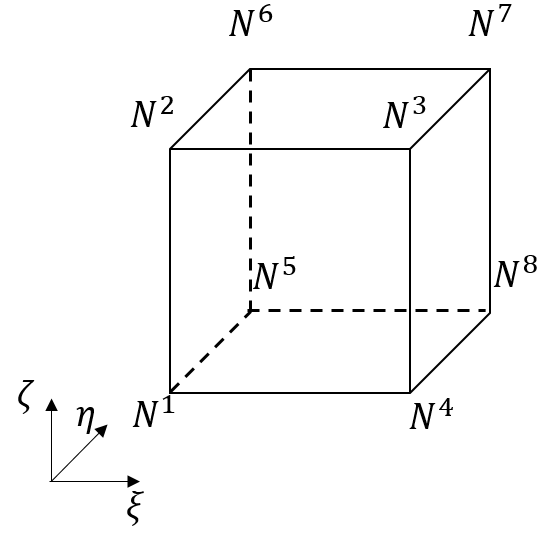
\includegraphics[width=6cm]{chap01/elemento_base.png} 
\caption{Elemento base (Domínio $\Omega^\xi$)}
\end{figure}



A associação de um ponto em $\Omega^\xi$ em um ponto em $\Omega^e$ é feito através da equação \ref{eq:isoparametrico}.


\begin{equation}
\label{eq:isoparametrico}
\mathbf{x}(\xi, \eta, \zeta) = \sum_{A=1}^{8} N_A(\xi, \eta, \zeta) \mathbf{x^e_A} 
\end{equation}

Assim, pode-se aplicar a mudança de variável na integral da equação \ref{eq:ae_def} para o domínio $\Omega^\xi$.

\begin{equation} 
 a_e(\phiix,\phijx) = \omeeint{S^T\phiix D S\phijx} = \omeint[\Omega^\xi]{S^T N^i D S N^j |J|}
\end{equation}


\begin{equation} 
 a_e(\phiix,\phijx) = \int^1_ {-1}\int^1_ {-1}\int^1_ {-1}{S^T N^i D S N^j |J|} \text{d}\xi \text{d}\eta \text{d}\zeta
\end{equation}

onde $J$ representa a matriz jacobiana. 

\begin{equation}
J = \begin{bmatrix}
\dxi[x]   &   \dxi[y] &   \dxi[z] \\
\deta[x]  &  \deta[y] &  \deta[z] \\
\dzeta[x] & \dzeta[y] & \dzeta[z] 
\end{bmatrix}
\label{eq:jacobiano}
\end{equation}

O valor das derivadas do Jacobiano podem ser obtidas derivando a \ref{eq:isoparametrico}.


\begin{equation}\label{eq:dev_x_xi}
\dxi[x] = \sum^8_{A=1} \dxi[N_A] x^e_A
\end{equation}
\begin{equation}
\deta[x] = \sum^8_{A=1} \deta[N_A] x^e_A
\end{equation}
\begin{equation}
\dzeta[x] = \sum^8_{A=1} \dzeta[N_A] x^e_A
\end{equation}



Pode-se perceber também que os somatórios podem ser transformados como a multiplicação de uma matriz linha por uma matriz coluna transformando, por exemplo, \ref{eq:dev_x_xi} em \ref{eq:dev_x_xi_matriz}.

\begin{equation}\label{eq:dev_x_xi_matriz}
\dxi[x] = 
\begin{bmatrix}
 \dxi[N^1]   & \dxi[N^2] & \cdots & \dxi[N^8]
\end{bmatrix}
\begin{bmatrix}
x^1    \\ 
x^2    \\ 
\vdots  \\ 
x^8  
\end{bmatrix}
\end{equation}

Com isso, substituindo em \ref{eq:jacobiano} as equações analógas a \ref{eq:dev_x_xi_matriz} para cada uma das entradas do jacobiano é possível obter a equação \ref{eq:jacobiano_prod}.


\begin{equation}\label{eq:jacobiano_prod}.
J = \der
\begin{bmatrix}
x^1 & y^1 & z^1 \\ 
x^2 & y^2 & z^2 \\ 
\vdots & \vdots  & \vdots  \\ 
x^8 & y^8 & z^8 \\ 
\end{bmatrix}
\end{equation}


